% A template for problem sets 
\documentclass[12pt,letterpaper]{article} 
\usepackage{listings}
\usepackage{fancyhdr} 
\usepackage{pdfpages}

\usepackage{wrapfig}
\usepackage{graphicx}
\graphicspath{{figures/}}
\usepackage[margin=1in,top=1.5in,headheight=3em]{geometry} 
\pagestyle{fancy}
\pagenumbering{roman}

\lhead{
	Advances in Computer Vision \\
	Problem Set 3
}
\rhead{
	Suman Nepal \\
	\today
}

\begin{document}
	
	\section*{Problem 1}
	
	\subsection*{(a)}
	I computed the change in phase angle in the FFT domain  and added the magnified change to the phase angle of the image 1 to get the final angle of the magnified image.Finally I inverse transformed of the complex numbers corresponding to the final magnified phase angle to get the magnified image.
	
	\begin{lstlisting}
	
phaseShift = angle(im2Dft) - angle(im1Dft);
magnification = angle(im1Dft) + magnificationFactor * phaseShift;
[m,n] = pol2cart(magnification, abs(im1Dft))
magnified = ifft2(complex(m,n));

	\end{lstlisting}
    The resulting image from the magnification is given below.
	\begin{figure}[htbp]
		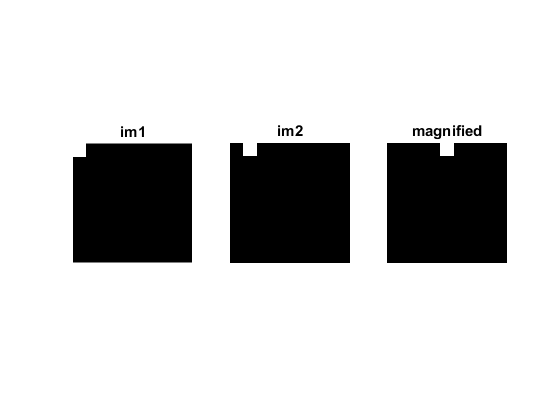
\includegraphics{parta.png}
		\caption{1D motion magnification}
	\end{figure}
	
	\subsection*{(b)}
	The resulting image from running part b is given below.
	\begin{figure}[htbp]
		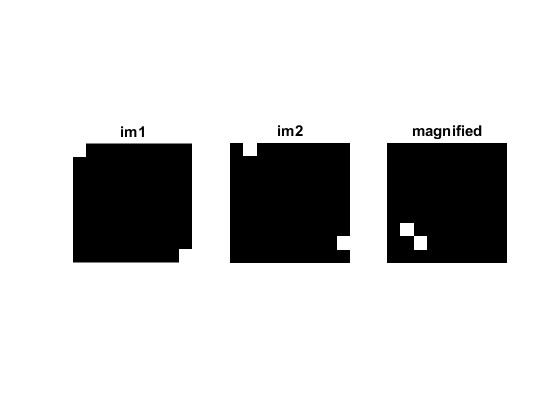
\includegraphics{partb.png}
		\caption{2d motion magnification}
	\end{figure}
There is two direction of motion in these images and phase shift due to each of the motion are applied to another one. The local changes in position is lost in the frequency domain and results in both horizontal and vertical shifts in the positions of both objects. 
Restricting the FFT to the local region and taking smaller patches of magnification helps in resolving this issue. This avoids changes due to motions in non local regions.
	\subsection*{(c)}
	I multiplied both of the images with the gaussian mask and doing the magnificaiton in each iteration.The relevant code for the method is given below:
	
\begin{lstlisting}
gaussianMask = exp((-(X-x).^2 - (Y- y).^2)/ (2 * sigma ^2 ));
im11 = im1.*gaussianMask;
im22 = im2.*gaussianMask;
windowMagnified = magnifyChange(im11, im22, magnificationFactor);
magnified = magnified + windowMagnified;

\end{lstlisting}

The resulting image from the magnification is given below.
\begin{figure}[htbp]
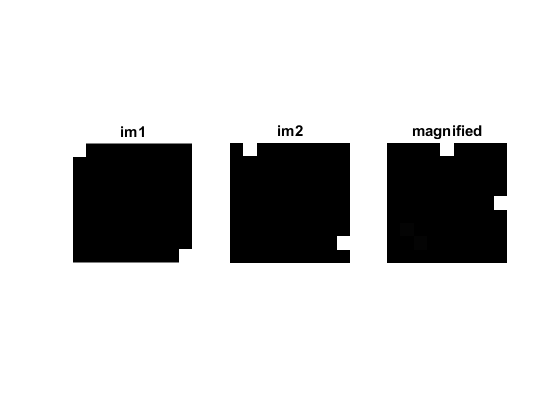
\includegraphics{partc.png}
\caption{Corrected 2D motion magnification using local gaussian mask}
\end{figure}

\subsection*{(d)}
The video magnification was achieved by following code. 
\begin{lstlisting}
%line 49 
gaussianMask = exp((-(X-x).^2 - (Y- y).^2)/ (2 * sigma ^2 ));

%magnify phase shift
windowMagnifiedPhase = windowAveragePhase + windowPhaseShift * magnificationFactor;
[m,n] = pol2cart(windowMagnifiedPhase, abs(windowDft));

windowMagnifiedDft = complex(m,n);
windowMagnified = abs(ifft2(windowMagnifiedDft));

\end{lstlisting}

\section*{(2)}
\subsection*{(a)}
\subparagraph*{(i)}

We know that
\begin{equation}
\textbf{$ C_{RGB} = T C_{XYZ}$}
\end{equation}  
We can multiply the $C_{XYZ}$ with T to get$ C_{RGB}$. We get the following plot when we plot the result.
\begin{figure}[htbp]
	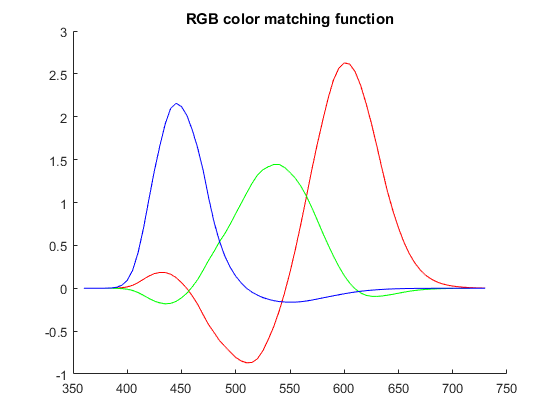
\includegraphics{rgb.png}
	\caption{RGB color matching function}
\end{figure}

From the figure, we can see that the color matching functions are not always positive. Different curve show different range of negativeness. The red color matching function, for instance is negative from wavelengths of 450 to 550 nm. Similarly for blue and green functions, we can see different negative regions. 

\subparagraph*{(ii)}
We know that $ C_{RGB}. P = I$ . Taking the pseudo inverse of the matrix $C_{RGB}$ we can get the primary light spectra. 
\begin{figure}[htbp]
	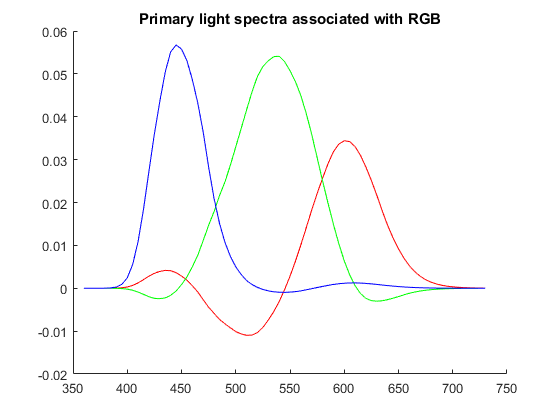
\includegraphics{rgbinv.png}
	\caption{RGB primary light spectra}
\end{figure}

As like the color matching functions, these light spectra are also negative in some region. The red spectra is negative between 450nm and 550 nm. Similary, green and blue primary spectra also have their respective negative regions. 
\subparagraph*{(iii)}

Plotting the CIE we get the following graph at figure 6.
\begin{figure}[htbp]
	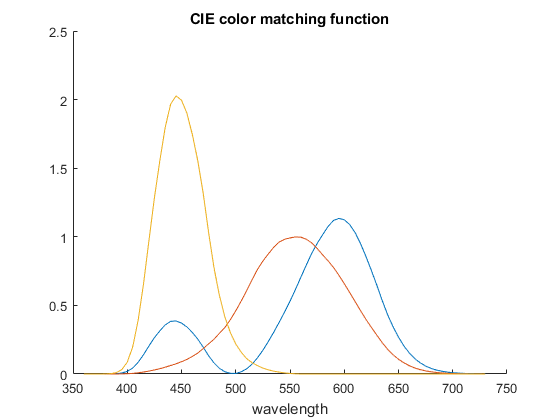
\includegraphics{cie.png}
	\caption{CIE color matching function}
\end{figure}

We can see that the curves do not have the negative regions. This is not a coincidence as it was specifically designed to be such.

\subparagraph*{(iv)}
\begin{figure}[htbp]
	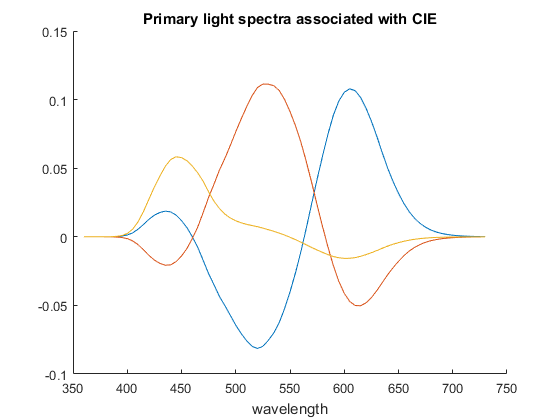
\includegraphics{cieinv.png}
	\caption{CIE color primary light spectra}
\end{figure}
As like before, we take the pseudo inverse of the CIE colormatching function. We get the following graph at figure 7. We can also see that the primaries are not always positive. We can see a large negative region on the blue spectrum between 450 and 550 nm wavelength. This is in contrast to negative region of red wavelength in RGB primary.
Similarly, red and yellow also have some negative region as seen in the plot.

\subsection*{(b)}
Each primary spectrum in Figure 8 has negative region. For example, the blue curve has it's negative range from 450 nm to 550 nm whereas yellow has negative range from 550nm to 700nm. 
\begin{figure}[htbp]
	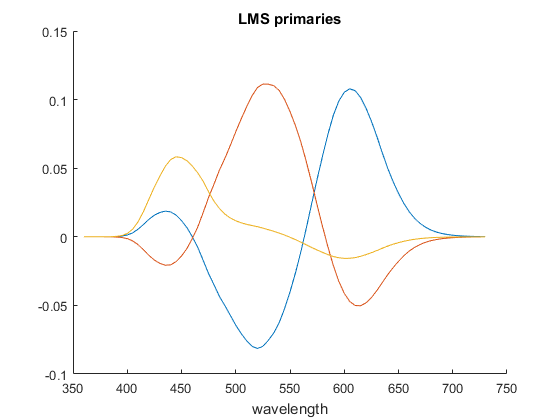
\includegraphics{lmsprimaries.png}
	\caption{LMS Primaries}
\end{figure}
\subsection*{(C)}

Let the non negative spectral response curves be L, M and S.We denote their components as $l_{1}, m_{1}, ... $. We define P as shown below which is also a non negative matrix as it contains all the positive numbers in C divided by a normalization constant. We showed that the particular arrangement when multiplied with C gives I, due to orthogonality properties of L, M and S.   
\begin{figure}[htbp]
	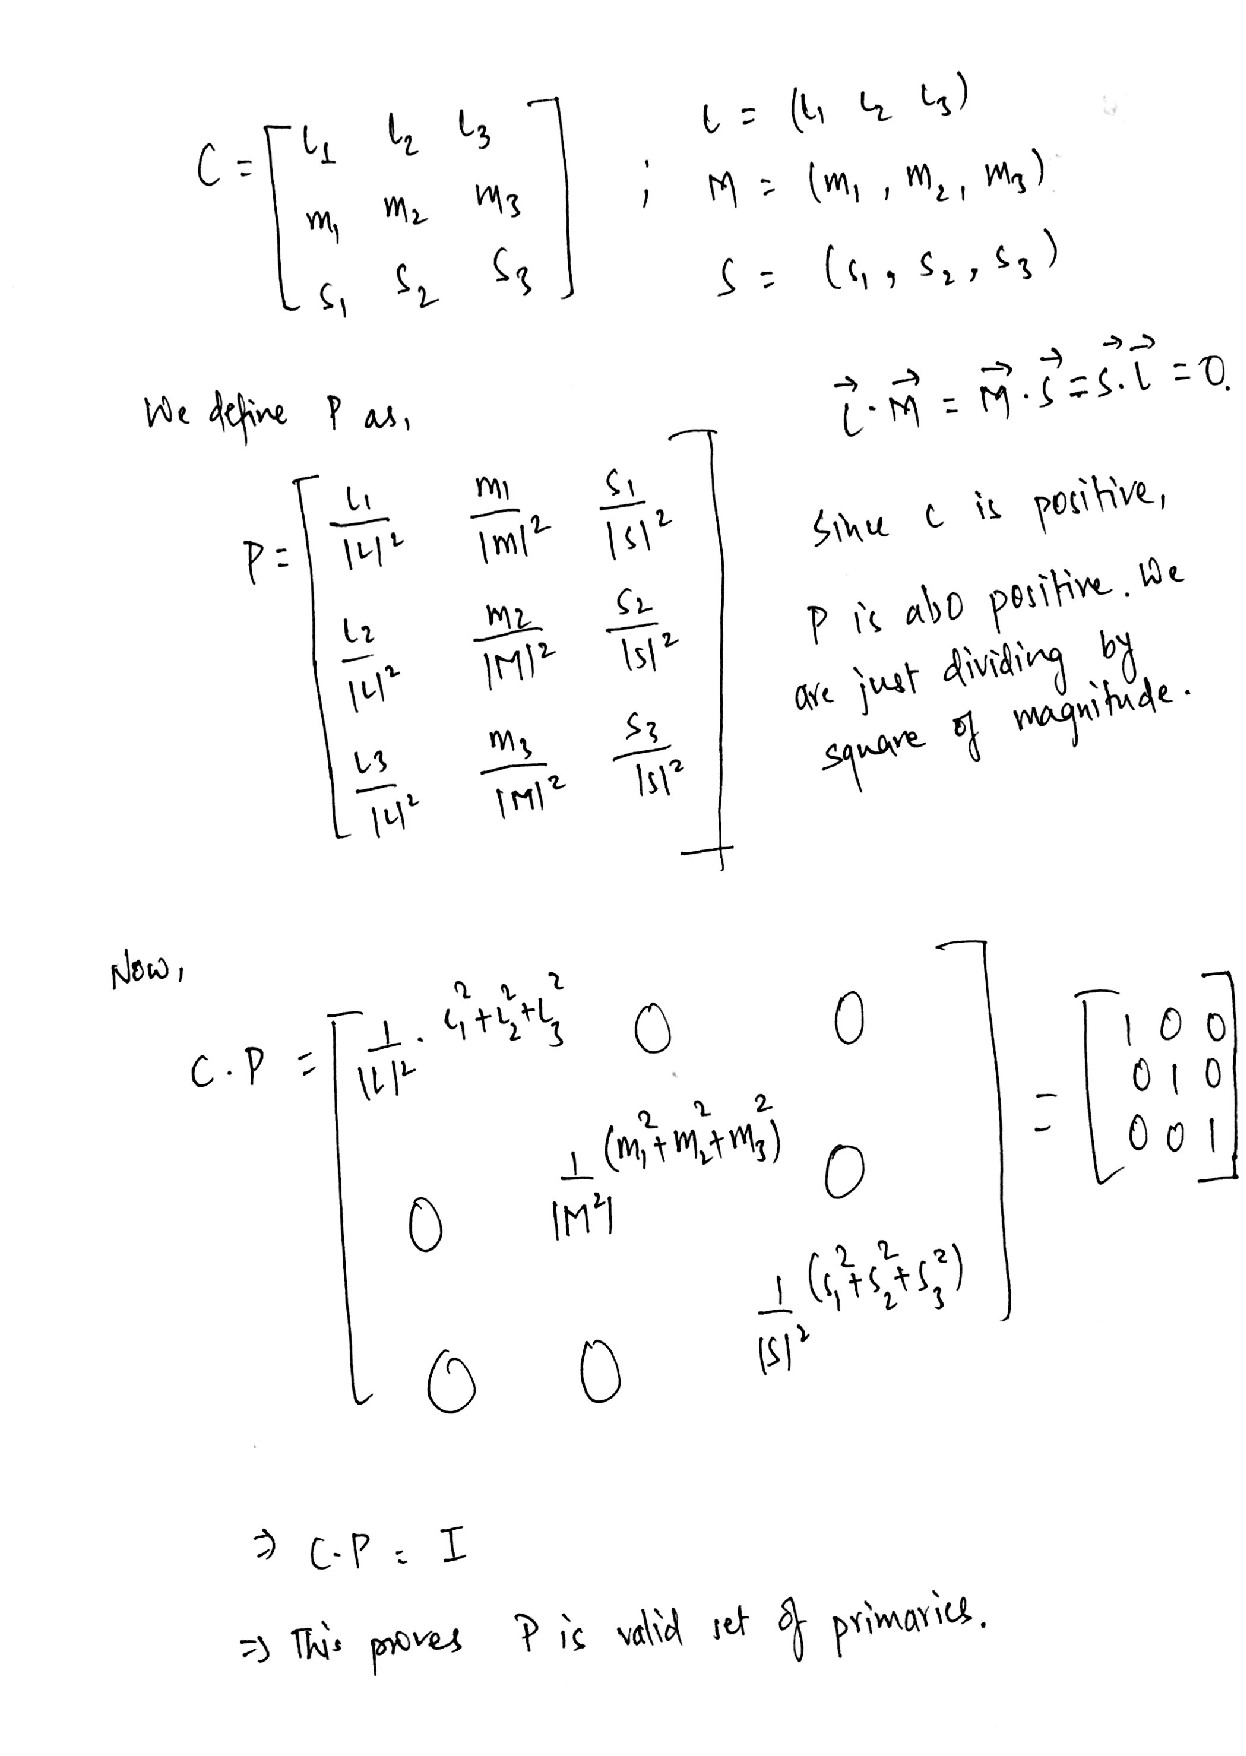
\includegraphics[width=\textwidth]{2c.pdf}
\end{figure}


\subsection*{d}

We cannot uniquely determine the  associated primaries P for a given color matching functions C. 

If y is a vector in null space of C, then \[        C .(inv(C) + k * [y, y, y]) = I         \]

        
 for all scaler values of k. This means I can have more than one P that give I when left multiplied by C. 

However, the opposite is true for the uniquely determined P. We can always find a unique C associated with P.From the above equation, it follows that every P has to be in form of 
\[   inv(C) + k * [y, y, y])  \] 
.Also, from uniqueness of left side inverse of matrix  inv(C), we can conclude that only one C can reduce inv(C) to I and k*[y y y] to 0 to result on CP = I.

\end{document}